%! alt Triangle ABC with side BC along the bottom. Ten circles of radius 1 sit in a row along BC, each touching BC and the next one; the first touches AB and is centred at B', and the last touches CA and is centred at C'. A circle of radius 1 centred at A' touches AB and CA. The triangle A'B'C', with B'C' = 18, C'A' = 20 and A'B' = 34, has its sides parallel to those of ABC at distance 1; it has area 144 and inradius 4, and ABC has inradius 5 and area 225.
%! after_paragraph 1
%! scale 1/4.4
% The shared preamble of every Cevian figure. pipeline/figures turns these colours into theme-aware paint,
% and refuses any other colour, so draw only with them:
%   figink (lines and labels), figaux (construction lines), figaccent (the object the argument turns on),
%   figtint and figaccenttint (light fills).
\documentclass[border=1.5pt]{standalone}
\usepackage{tkz-euclide}
\definecolor{figink}{RGB}{0,0,0}
\definecolor{figaux}{RGB}{85,85,85}
\definecolor{figaccent}{RGB}{192,57,43}
\definecolor{figtint}{RGB}{221,221,221}
\definecolor{figaccenttint}{RGB}{245,213,208}
% tkz-euclide's defaults draw circles, compasses and marks in 50% grey and fill points with a tint.
\makeatletter
\def\tkz@otherlinecolor{figink}
\def\tkz@euc@circlecolor{figink}
\def\tkz@euc@compasscolor{figink}
\def\tkz@euc@mkcolor{figink}
\def\tkz@mk@fill{figink}
\def\tkz@euc@pointfillcolor{figink}
\makeatother
\tkzSetUpLine[color=figink,line width=.7pt]
\tkzSetUpArc[color=figink,line width=.7pt]
\tkzSetUpCompass[color=figink,line width=.5pt]
\tkzSetUpPoint[color=figink,fill=figink,size=3.1pt]
\tikzset{
  every picture/.style={line cap=round,line join=round,color=figink},
  circle style/.append style={color=figink,line width=.7pt},
  aux/.style={color=figaux,line width=.45pt,dash pattern=on 2.6pt off 2pt},
  key/.style={color=figaccent,line width=1pt},
  mk/.style={color=figink,line width=.5pt},
  lbl/.style={color=figink,inner sep=2.2pt},
  len/.style={color=figink,inner sep=1.5pt,font=\small},
}

\begin{document}
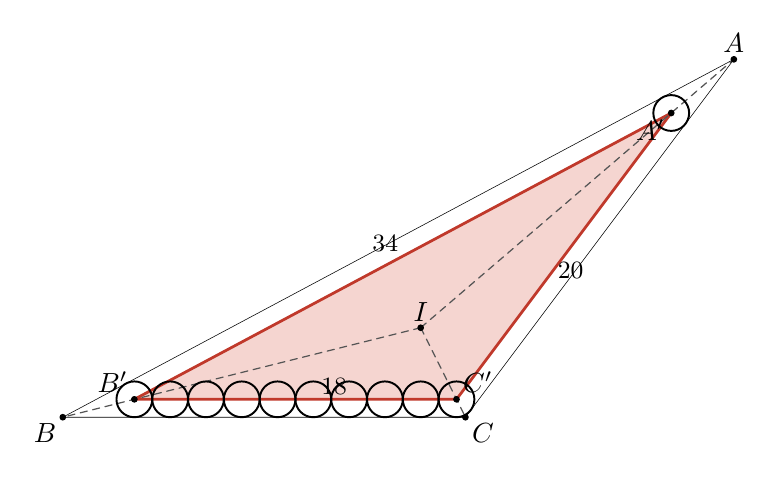
\begin{tikzpicture}
\tkzDefPoint(7.6136364,4.3181818){A} %! A = (33.5, 19)
\tkzDefPoint(-0.90909091,-0.22727273){B} %! B = (-4, -1)
\tkzDefPoint(4.2045455,-0.22727273){C} %! C = (18.5, -1)
\tkzDefPoint(6.8181818,3.6363636){Ap} %! Ap = (30, 16)
\tkzDefPoint(0.0,0.0){Bp} %! Bp = (0, 0)
\tkzDefPoint(4.0909091,0.0){Cp} %! Cp = (18, 0)
\tkzDefPoint(3.6363636,0.90909091){I} %! I = (16, 4)
\tkzDefPoint(0.45454545,0.0){O1} %! O1 = (2, 0)
\tkzDefPoint(0.90909091,0.0){O2} %! O2 = (4, 0)
\tkzDefPoint(1.3636364,0.0){O3} %! O3 = (6, 0)
\tkzDefPoint(1.8181818,0.0){O4} %! O4 = (8, 0)
\tkzDefPoint(2.2727273,0.0){O5} %! O5 = (10, 0)
\tkzDefPoint(2.7272727,0.0){O6} %! O6 = (12, 0)
\tkzDefPoint(3.1818182,0.0){O7} %! O7 = (14, 0)
\tkzDefPoint(3.6363636,0.0){O8} %! O8 = (16, 0)
\tkzDefPoint(0.0,-0.22727273){T0} %! T0 = (0, -1)
\tkzDefPoint(0.45454545,-0.22727273){T1} %! T1 = (2, -1)
\tkzDefPoint(0.90909091,-0.22727273){T2} %! T2 = (4, -1)
\tkzDefPoint(1.3636364,-0.22727273){T3} %! T3 = (6, -1)
\tkzDefPoint(1.8181818,-0.22727273){T4} %! T4 = (8, -1)
\tkzDefPoint(2.2727273,-0.22727273){T5} %! T5 = (10, -1)
\tkzDefPoint(2.7272727,-0.22727273){T6} %! T6 = (12, -1)
\tkzDefPoint(3.1818182,-0.22727273){T7} %! T7 = (14, -1)
\tkzDefPoint(3.6363636,-0.22727273){T8} %! T8 = (16, -1)
\tkzDefPoint(4.0909091,-0.22727273){T9} %! T9 = (18, -1)
\tkzDefPoint(7.0454545,3.6363636){Ta} %! Ta = (31, 16)
%! fact dist(Bp, Cp) == 18
%! fact dist(Cp, Ap) == 20
%! fact dist(Ap, Bp) == 34
%! fact tangent(Bp, 1, A, B)
%! fact tangent(Bp, 1, B, C)
%! fact tangent(Cp, 1, C, A)
%! fact tangent(Cp, 1, B, C)
%! fact tangent(Ap, 1, A, B)
%! fact tangent(Ap, 1, C, A)
%! fact parallel(Bp, Cp, B, C)
%! fact parallel(Cp, Ap, C, A)
%! fact parallel(Ap, Bp, A, B)
%! fact collinear(I, A, Ap)
%! fact collinear(I, B, Bp)
%! fact collinear(I, C, Cp)
%! fact area(Ap, Bp, Cp) == 144
%! fact inradius(Ap, Bp, Cp) == 4
%! fact inradius(A, B, C) == 5
%! fact area(A, B, C) == 225
%! fact dist(Bp, O1) == 2
%! fact dist(O8, Cp) == 2
\tkzFillPolygon[color=figaccenttint](Ap,Bp,Cp)
\tkzDrawPolygon(A,B,C)
\tkzDrawPolygon[key](Ap,Bp,Cp)
\tkzDrawSegments[aux](I,A I,B I,C)
\tkzDrawCircle(Bp,T0)
\tkzDrawCircle(O1,T1)
\tkzDrawCircle(O2,T2)
\tkzDrawCircle(O3,T3)
\tkzDrawCircle(O4,T4)
\tkzDrawCircle(O5,T5)
\tkzDrawCircle(O6,T6)
\tkzDrawCircle(O7,T7)
\tkzDrawCircle(O8,T8)
\tkzDrawCircle(Cp,T9)
\tkzDrawCircle(Ap,Ta)
\tkzDrawPoints(A,B,C,Ap,Bp,Cp,I)
\tkzLabelPoint[above,lbl](A){$A$}
\tkzLabelPoint[below left,lbl](B){$B$}
\tkzLabelPoint[below right,lbl](C){$C$}
\tkzLabelPoint[below left,lbl](Ap){$A'$}
\tkzLabelPoint[above left,lbl](Bp){$B'$}
\tkzLabelPoint[above right,lbl](Cp){$C'$}
\tkzLabelPoint[above,lbl](I){$I$}
\tkzLabelSegment[above,pos=.62,len](Bp,Cp){$18$}
\tkzLabelSegment[right,pos=.45,len](Cp,Ap){$20$}
\tkzLabelSegment[above left,pos=.5,len](Ap,Bp){$34$}
\end{tikzpicture}
\end{document}
